\documentclass[12pt, a4paper]{beamer}

\usetheme{Hannover}
\usecolortheme{whale}

\begin{document}
	\setbeamertemplate{sidebar left}{}
	\title{Progress Presentation-I}
	\subtitle{e-Yantra Summer Internship-2018 \\ CNC for GrowBox}
	\author{Devang Joshi\\Ujwal Pawar\\Harsh Lunia\\
	Mentor: \\Lohit Penubaku,\\Ajit and\\Kedar}
	\institute{IIT Bombay}
	\date{\today}
	%\addtobeamertemplate{sidebar left}{}{\includegraphics[scale = 0.3]{logowithtext.png}}
	\frame{\titlepage}

\setbeamertemplate{sidebar left}[sidebar theme]
\section{Overview of Project}
\begin{frame}{Overview of Project}

		\centering \LARGE \underline {CNC for GrowBox}

\end{frame}	

\begin{frame}
		\centering {\Large {\underline {Objective}:-}}
		\begin{itemize} \vspace{2mm}
			\item Understanding the requirements and analysing the existing GrowBox
			\item Designing of spray and seeding mechanism
			\item Monitoring plant growth using IP techniques and ML if needed. 
			\item Complete system integration and testing 
		\end{itemize}
\end{frame}	

\begin{frame}
		\centering {\Large {\underline {Deliverables}:-}}
		\begin{itemize} \vspace{2mm}
			\item Working CNC fixed inside the GrowBox
			\item IP for XY mapping and plant monitoring
			\item Documentation of CNC design and IP codes
		\end{itemize}
\end{frame}	

\section{Overview of Task}
	\begin{frame}{Overview of Task}
\begin{table}[htbp]
  \centering
  \tiny
    \begin{tabular}{clrc}
    \multicolumn{1}{p{2em}}{\textbf{Task No.}} & \multicolumn{2}{c}{\textbf{Task}} & \textbf{Deadline} \\
          & \multicolumn{1}{c}{\textbf{Mechanical}} & \multicolumn{1}{c}{\textbf{Electronic/Computer Science}} &  \\
          & \multicolumn{2}{c}{\textbf{Week 1}} &  \\
    1     & \multicolumn{2}{l}{Understanding the requirements and analysing the existing GrowBox} & 1 days \\
    2     & \multicolumn{1}{p{13.57em}}{Modeling/Designing the 1st iteration of the CNC to fit inside the GrowBox} & \multicolumn{1}{p{13.57em}}{Literature survey on existing IP for plant monitoring and using IP to transform trough dimensions to XY for CNC} & 4days \\
          & \multicolumn{2}{c}{\textbf{Week 2}} &  \\
    3     & \multicolumn{1}{p{13.57em}}{Analysing the designs in Ansys, considering all the parameters.} & \multicolumn{1}{p{13.57em}}{Setting up the base system for image processing on Rpi and ML machine} & 3 days \\
    4     & \multicolumn{1}{p{13.57em}}{Designing of spray and seeding mechanism} & \multicolumn{1}{p{13.57em}}{Testing the system to run minimal problems which may be faced} & 2 days \\
          & \multicolumn{2}{c}{\textbf{Week 3}} &  \\
    5     & \multicolumn{2}{l}{Construction of the design and testing of CNC} & 2 days \\
    6     & \multicolumn{2}{l}{Interfacing and writing code for CNC} & 3 days \\
    \end{tabular}%
  \label{tab:addlabel}%
\end{table}%
\end{frame}

\section{Task Accomplished}
	\begin{frame}{Task Accomplished}

% Table generated by Excel2LaTeX from sheet 'Sheet1'
\begin{table}[htbp]
  \centering
  \tiny
    \begin{tabular}{cp{12em}l}
    \textbf{Sr.No.} & \multicolumn{1}{c}{\textbf{Mechanical}} & \multicolumn{1}{c}{\textbf{Electronics/Computer Science}} \\
    1     & Finalised all the mechanism for the motion of CNC in all the required direction. & Reading of literature pertaining to image processing. \\
    2     & Finished selecting various materials according to there properties suitable for the machine parts. & \multicolumn{1}{p{24.43em}}{Detecting of green trough and subsequently boxing the trough in a rectangle to generate a grid which divides the whole trough into plantable free spaces for each plant.} \\
    3     & Done analysis on the Ansys software to find the required strength of the part and factor of safety. & \multicolumn{1}{p{24.43em}}{Installed and configured Rasbian Stretch on provided rasberry pi.} \\
    4     & Prepared a material requirement list with estimated price for the construction of CNC. & Ardino and OpenCV was installed on the above board. \\
    \end{tabular}%
  \label{tab:addlabel}%
\end{table}%

\end{frame}

	\begin{frame}
		\begin{figure}
		\begin{center}
		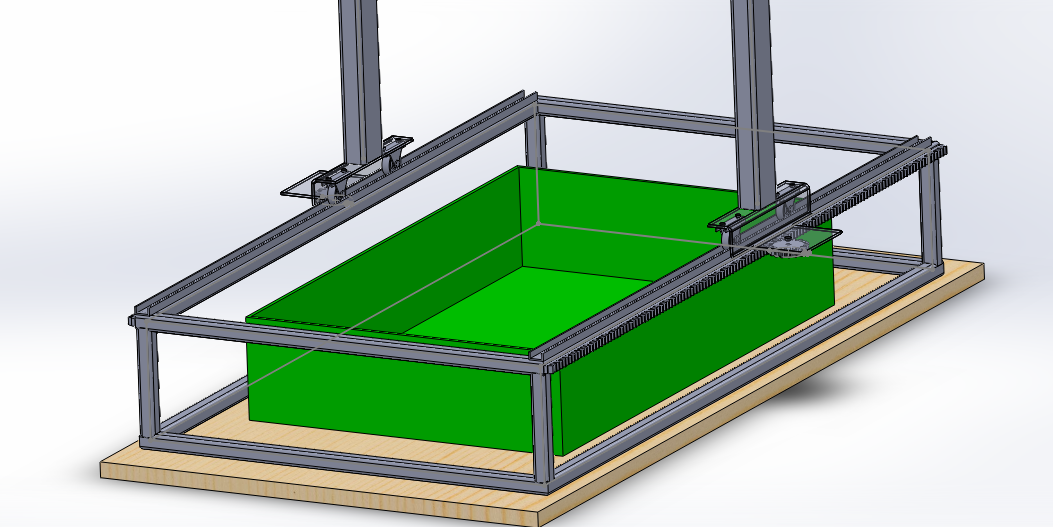
\includegraphics[width=\textwidth]{1.png}
		\caption{1st week x-direction motion}
		\end{center}
		\end{figure}
	\end{frame}
	
	\begin{frame}
		\begin{figure}
		\begin{center}
		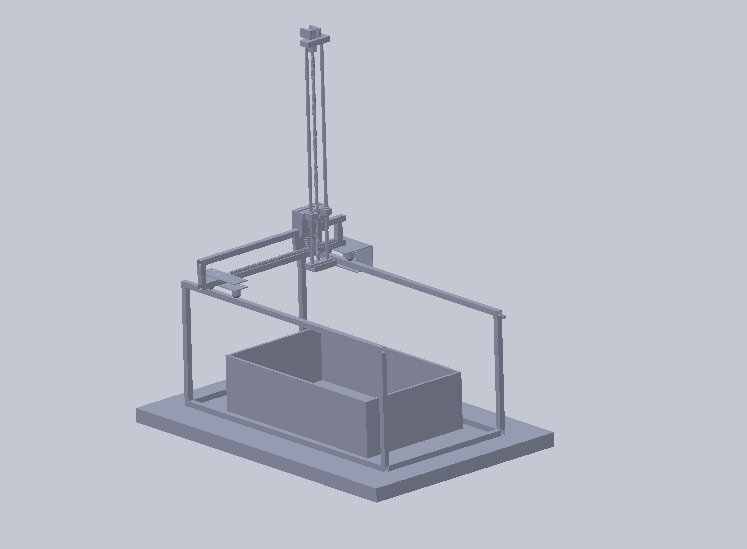
\includegraphics[width=0.8\textwidth]{1stweekdesign.jpg}
		\caption{1st week all direction motion}
		\end{center}
		\end{figure}
	\end{frame}

	\begin{frame}
		\begin{figure}
		\begin{center}
		
\includegraphics[width=0.8\textwidth]{heavy.jpg}
		\end{center}
		\end{figure}
	\end{frame}

	\begin{frame}
		\begin{figure}
		\begin{center}
		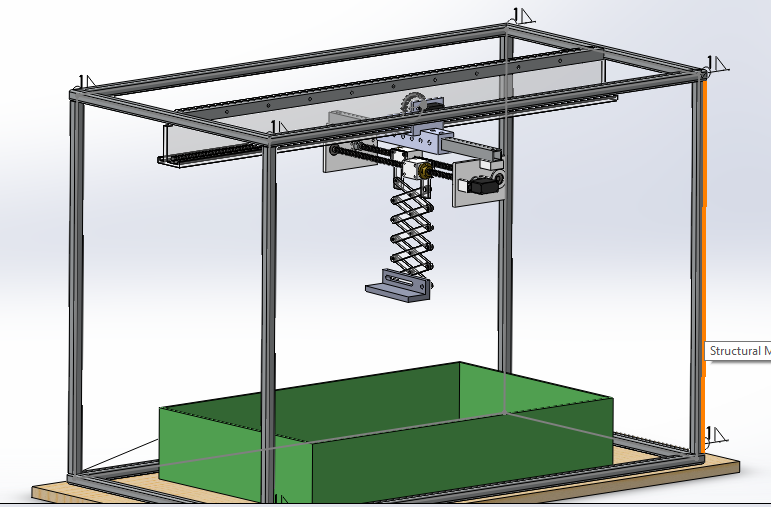
\includegraphics[width=0.9\textwidth]{2.png}
		\caption{2nd week all direction motion}
		\end{center}
		\end{figure}
	\end{frame}

	\begin{frame}
		\begin{figure}
		\begin{center}
		
\includegraphics[width=0.9\textwidth]{unreach.png}
		\end{center}
		\end{figure}
	\end{frame}

	\begin{frame}
		\begin{figure}
		\begin{center}
		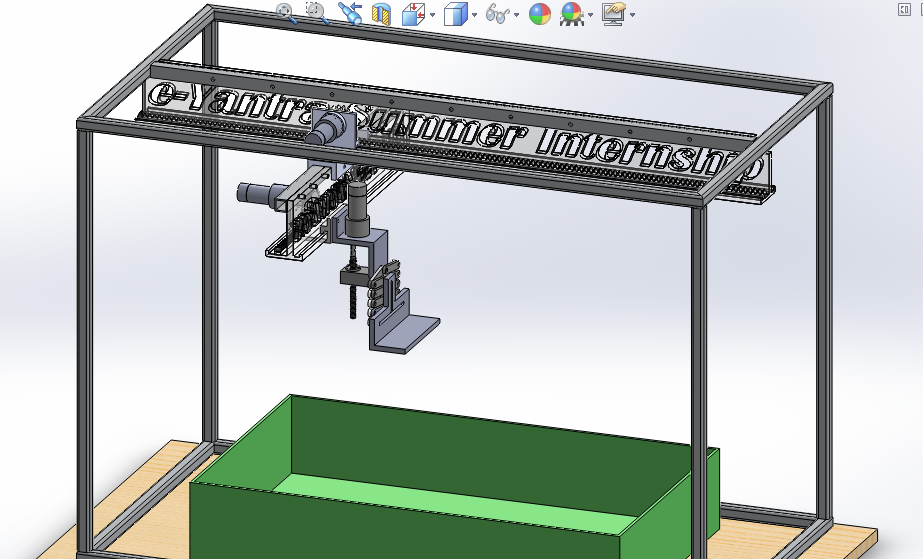
\includegraphics[width=0.9\textwidth]{3.png}
		\caption{Final model}
		\end{center}
		\end{figure}
	\end{frame}

	\begin{frame}
		\begin{figure}
		\begin{center}
		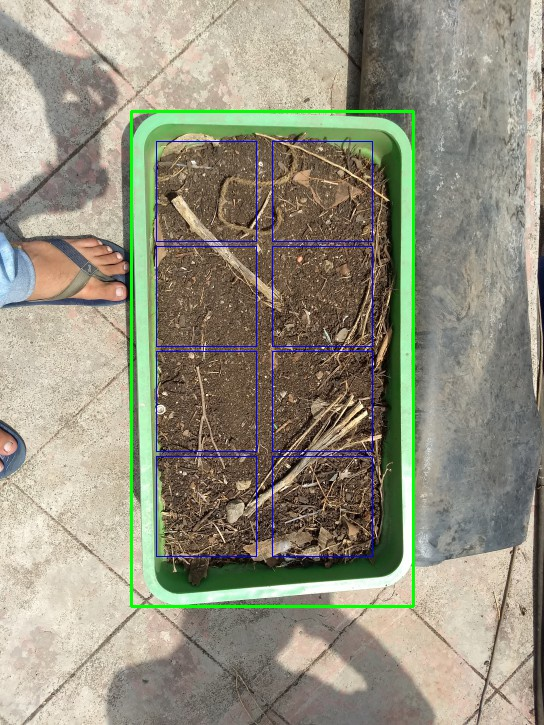
\includegraphics[ angle=90,width=0.9\textwidth]{grid.jpg}
		\caption{Sample grid generation}
		\end{center}
		\end{figure}
	\end{frame}

	\begin{frame}
		\begin{figure}
		\begin{center}
		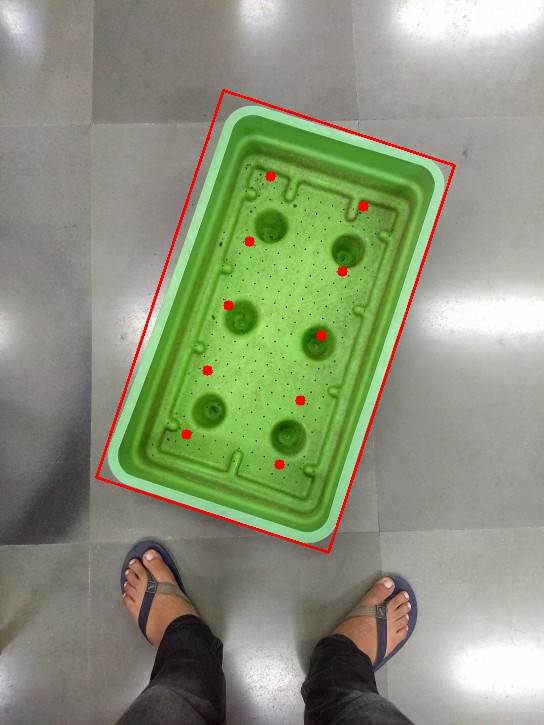
\includegraphics[ angle=90,width=0.9\textwidth]{dynamic.jpg}
		\caption{Dynamic sample grid generation}
		\end{center}
		\end{figure}
	\end{frame}

\section{Challenges Faced}
\begin{frame}{Challenges Faced}
	\centering{\textbf{Mechanical}}
	\begin{itemize}
		\item Firstly, we find difficulty in finding the requirements or necessary constraints of the project.
		\item To obtain the transferability from one box to another one.
		\item To design such a light weight and compact mechanisms to meet the requirements.
		\item To design an overhanging mechanism.
		\item Designing expandable mechanism for the vertical motion which occupies the least space.
	\end{itemize}
\end{frame}

\begin{frame}
	\centering{\textbf{Electronic/Computer Science}}
	\begin{itemize}
		\item Dynamic grid generation that has to be independent of the orientation of trough w.r.t the box. 
		\item Initialisation of coordinate system for CNC to receive commands after processing the images clicked by pi camera.
		\item At the fixed height of grow box, pi camera isn't able to capture whole of trough in one click.
	\end{itemize}
\end{frame}

\section{Future Plans}
\begin{frame}{Future Plans}
	\centering{\textbf{Mechanical}}
	\begin{itemize}
		\item Designing of spray and seeding mechanism
		\item Construction of the CNC.
		\item Testing the functioning of all the mechanism.
	\end{itemize}
\end{frame}

\begin{frame}
	\centering{\textbf{Electronics and Computer Science}}
	\begin{itemize}
		\item To implement the decided coordinate system initialisation procedure.
		\item To process the whole of grow box by clicking multiple images and determine the position of trough, consequently the grid points
		\item To read literature and implement an algorithm to estimate moisture content on each plant.  
	\end{itemize}
\end{frame}

\section{Thank You}
\begin{frame}{Thank You}
	\centering THANK YOU !!!
\end{frame}
\end{document}
